\newpage
\section{Physical threats and counter measures}

\subsection{Physical threat}


Vocabulary: in some part of the literature can be found standard expression 
like 'exponent blinding' and 'message masking', we will consider blinding and masking 
as perfect synonymous considering that the expression 'exponent masking' make sense.

an intro better than :

Frequently in so-called 'bullet proof  programming' all important parameters such as
an RSA modulus can be stored many times with different mask, and after that their integrity have been checked, one modulus of the xored modulus is transformed 
to an arithmetic masked modulus, and then is ready for use.
\vspace{3mm}
Algorithms have been setup to securely switch from one type of masking another.
Quiqskatter in the 2000's or more recently: 
"Debraize - efficient and provably secure methods from switching from arithmetic from boolean masking - CHES2012"\footnote{ Do you know any use of a boolean masking in a asymmetrical crypto stuff? If yes communicate! }

\subsubsection{Counter measures to side channel}

\begin{center}
\large
Boolean masking: $ x = x \oplus m $\\
Arithmetic masking: $ x = (x - m)$ mod $2^k$ \\
\normalsize
\end{center}

The following countermeasures \textbf{rely on the arithmetic masking scheme}:
using some classical mathematics identities, the result is computed in a 
way which is not the  most natural neither the quicker. 

Transparent Countermeasure: Exponent blinding, ...\\
Non Transparent Countermeasure: Multiplicative Message blinding, ...\\

\begin{itemize}
\item	\begin{tabularx}{\linewidth}{ p{16cm} p{1.5cm}}
		Exponent blinding -\textit{Coron Ches'1999}-  & $0\%$ \\ 
		\end{tabularx}	
		\noindent 
		The direct computation: $c = m^e$ mod $n$ is replaced by a random one:
			\begin{center}
			$c = m^{e+r \times \phi (n) }$ mod $n$\\
		\end{center}
		Also known as \textit{'Coron's first Countermeasure'} where $r$ is a random number, the result is not changed thanks to Euler's theorem that is to be changed for each encryption, this countermeasure will impact the number of bits of the exponent, and then the number of visible patterns.

		Practical remarks: 
		\begin{center}
			\textbf{$r$ shall be small to regard to $m$!}
		\end{center}

		Remarks: registers and transparency
		\begin{itemize}
			\item carefully note that if the intermediate computation are reduced modulo $n$
			then this countermeasure has strictly no effect. Intermediate computation will only be 
			masked when the register size would have been increased sufficiently.
			\item When the masked result has been calculated then the correct result is 
			simply obtain by reduced modulo $n$. No special operation depending of the mask 
			have to be performed: this is a \textit{transparent mask}.
		\end{itemize}



\item	\begin{tabularx}{\linewidth}{ p{16cm} p{1.5cm}}
		Multiplicative Message blinding -\textit{Kocher' 1995}-  & $0\%$\\ 
		\end{tabularx}	
		\noindent 
		The direct computation: $c = m^e$ mod $n$ is replaced by a random one:
		\begin{center}
		$m^{'} = m \times r \mod n$\\
		$c^{'} = {m^{'}}^e \mod n$
		\end{center}
		Non transparent countermeasure: recover the original message need an extra operation
		\begin{center}
		$ c  = c^{'} \times {r}^{-e} \mod n$
		\end{center}

		Practical remarks: 
		\begin{center}
			\textbf{$r$ and $m$ share the same size !}
		\end{center}

		\newpage
		Remarks
		\begin{itemize}
			\item Computational cost of 'random numbers'\\
		Generation of a random mask $r$	and the extra exponentiation are expensive.
		Some manufacturer prefer to cheat a bit generating small numbers and from 
		them creating the 'random number' expected, thanks to some available transformation.
		(a 32 bytes 'random R' can be generate by example with $R = r^k \mod n$ from to 
		really random number of two bytes each)
		
			\item Note that a choice is possible to remove the mask at then 
			end of the signature forge or while verifying this one if the mask is available see Schaum's blind signature.
			
			\item an extra operation is required to recover the original signature: non transparent mask !		
		\end{itemize}
		
\item	\begin{tabularx}{\linewidth}{ p{16cm} p{1.5cm}}
		Additive Message blinding -\textit{}-  & $0\%$ \\ 
		\end{tabularx}	
		\noindent 
		The message is replaced by a random one:
		\begin{center}
			$m^{'} = m + r \times n \mod( k \times n$)\\
		\end{center}
		To obtain the desired signature a extra reduction is necessary:
		\begin{center}
			$ c = c^{'} \mod n$
		\end{center}
		
		Practical remarks: 
		\begin{center}
			\textbf{$r$ shall be small to regard to $m$ !}
		\end{center}
		
\item Exponent splitting.
pick-up a random $r$ and form $r^{\ast}=e-r$ and compute separately :
		\begin{center}
			$ S_{r} = m^{r} \mod n$ and $ S_{r^{'}} = m^{r^{'}} \mod n$,
		\end{center}
		Finally
		\begin{center}
			$S = S_{r} \times  S_{r^{'}} $
		\end{center}
		Practical remarks: 
		\begin{center}
			\textbf{$r$ and $m$ share the same size !}
		\end{center}
Splitting is considered to be a very secured solution against side channel:
\begin{itemize}
\item the implementation shall be SPA resistant
\item $r$ shall be small in regard of $e$
\end{itemize}		

\item	\begin{tabularx}{\linewidth}{ p{16cm} p{1.5cm}}
		Modulus blinding -\textit{C.Giraud ' 2006}-  & $0\%$ \\ 
		\end{tabularx}	
		\noindent 
		The modulus replaced by a random one:
		\begin{center}
			$n^{'} =  k \times n$
		\end{center}
		Once that the final result is obtained it is then reduced modulo $n$ 
		to unmask the result. Where $r$ is a random number, the result is not changed 
		thanks to Euler's theorem. If $r$ is changed frequently, on a Square and Multiply 
		Always implementation, this countermeasure will impact the number of bits of the 
		exponent, and then the number of burst.

\item	\begin{tabularx}{\linewidth}{ p{16cm} p{1.5cm}}
			Multiplicative Message blinding -\textit{kocher ??}-  & $0\%$ \\ 
			\end{tabularx}	
			\noindent 
The direct computation: $c = m^e \mod n$ is replaced by a random one:
\begin{center}
$c^{'} = (r \times m)^{ e } \mod n$\\
\end{center}
Exponentiate as usual, then remove the mask applying: $ f:x \rightarrow x/r^e$ mod $n$
	\begin{center}
		$c = {( r \times m )}^e / r^e$ mod $n$
	\end{center}

		Remarks:
		\begin{itemize}
			\item where $r$ is a random number, under the following conditions 
			exponent splitting is considered to be a very secured solution against 
			side channel: the implementation shall be SPA resistant and both new 
			exponents $e - r$, practically r is always small.
			\item the exponent can be split in much more than 2 parts...
			\item this double the time required to obtain the exponentiation...
		\end{itemize}

		\textbf{Important variants:} The famous 'Schaume Blind Signature'\\
This way to use this countermeasure, is more used for protocol reasons.
The interest is to have a protocol allowing a person to sign a blinded message:
the signature is genuine but the real data signed is blinded.
\begin{center}
$c^{\ast} = (r^d \times m )^{ e } \mod n = r \times m ^{ e } \mod n $\\
$m = {c^{\ast}}^d  \times  r^{-1}$
\end{center}

\end{itemize}

\subsubsection{Counter measures side channel: slowing down the exponentiation}
Algorithms presented in the previous subsection were only interested in being fast,
without particular concern about the side channel security, algorithms hereafter 
presented favourize the security on the efficiency.


\begin{itemize}
\item	\begin{tabularx}{\linewidth}{ p{16cm} p{1.5cm}}
			Randomized exponentiation -\textit{??}-  & $5\%$ \\ 
			\end{tabularx}	
			\noindent
The idea of this counter measure is to change regularly the type of algorithm 
used for exponentiation.

By example to use the binary method in LtoR and RtoL 
version 'alternatively', using a Random Number Generator.



\item	\begin{tabularx}{\linewidth}{ p{16cm} p{1.5cm}}
			Montgomery ladder technique -\textit{Messerge-Dabish-Sloan Ches'1999}-  & $0\%$ \\ 
			\end{tabularx}	
			\noindent
The idea of this counter measure is to change regularly the type of algorithm used for exponentiation.
By example to use the binary method in LtoR and RtoL version 'alternatively', using a Random Number Generator.



\item \begin{tabularx}{\linewidth}{ p{16cm} p{1.5cm}}
			Overlapping window methods -\textit{Itoh, Yajima, Takenaka, Tori Ches'2002}-  & $0\%$ \\ 
			\end{tabularx}	
			\noindent
The idea of this family of counter measures is to use the $2^k$-ary method in a redundant way.
In the normal $2^k$-ary method when a window is scanned and that the relative computation took place
the window is shift of $k$ bits. Here the idea is to shift the window of less than $k$ bits.\\
			\begin{figure}[h]
				\begin{center}
	        	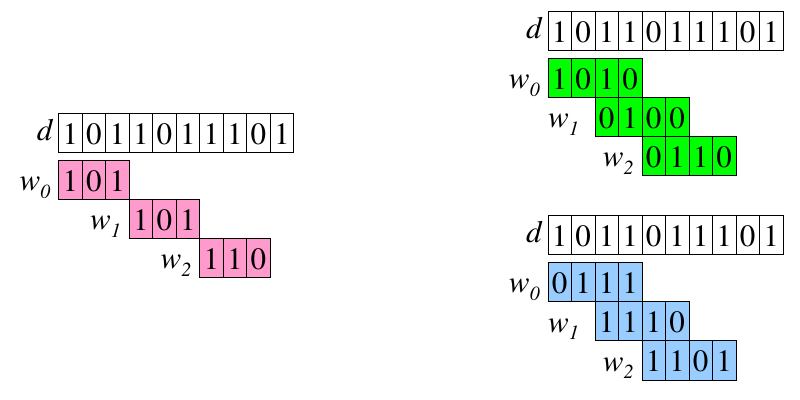
\includegraphics[scale=0.30]{images/Over.png}
				\caption{Overlapping window methods illustration}
				\end{center}
			\end{figure}

Let's assume that a $2^5$-ary method with an overlapp of $2$ bits: the window is each time shifted of $3$ 
bits instead of $5$. 
During the first exponentiation, the three first bits will be read and stored normally in the window but the two last bits will be two random ones,
and then the exponentiation of this window would take place.
At the next round of the exponentiation, this random will be compensate, and so on.

	
	  \item	\begin{tabularx}{\linewidth}{ p{16cm} p{1.5cm}}
			Clavier's square always method -\textit{Clavier 2011}-  & $0\%$ \\ 
			\end{tabularx}	
			\noindent
			Revisiting the Babylonians method replacing multiplications by squarings, thanks to 
			an old identity :
			\begin{center}			
				$x \times y = (\frac{x+y}{2})^2-(\frac{x-y}{2})^2$
			\end{center}
			It also has the advantage to be easily parallizable
			and it is always faster than Montgomery ladder technique. 
			In practice only atomic version of this technique should be used,
			can be optimized with a the sliding window method.
			\\

			\vspace{5mm}
			\textit{VS side channel cryptanalysis}\\
			immune against SvsM discrimination
			\vspace{5mm}
\end{itemize}





\subsubsection{Counter measures to fault injection}

\begin{itemize}
\item \begin{tabularx}{\linewidth}{ p{16cm} p{1.5cm}}
			Shamir's trick -\textit{1999}-  & $0\%$ \\ 
	  \end{tabularx}
	  \noindent A probabilistic test - \textit{e.g.} not always working - detecting if the 
	  forging has been faulted, the probability of detection increase with the length of $r$.
	  
		\begin{algorithm}[h]
			\KwIn{m, d, r, $r_p$ , $r_q$ , n}
			\KwOut{  $ y   =  x^d \mod n$, if genuine }
			 $ S_{r \times p}  =  m^e \mod r \times p$ \;
			 $ S_{r \times q}  =  m^e \mod r \times q$ 
			\If{ $S_{r \times p} \neq S_{r \times q \mod r}$ }
			{
			abort				
			}									 
			\Return{$ S = CRT(S_{r \times p}, S_{r \times q} ) $}\;
			\caption{Shamir's trick \textit{'Extend and reduce modulus'} }
		\end{algorithm}
		
		Remarks	
		\begin{itemize}
			\item Require the knowledge of $d$  -and not $d_p$, $d_q$-
			\item Does not detect fault during the recombination stage
			\item significantly longer exponentiation
		\end{itemize}	

\item \begin{tabularx}{\linewidth}{ p{16cm} p{1.5cm}}
			A faster countermeasure -\textit{1999}-  & $0\%$ \\ 
	  \end{tabularx}
	  \noindent A probabilistic test - \textit{e.g.} not always working - detecting if the 
	  forging has been faulted, the probability of detection increase with the length of $r$.
	  
		\begin{algorithm}[h]
			\KwIn{m, d, r, $r_p$ , $r_q$ , n}
			\KwOut{  $ y   =  x^d \mod n$, if genuine }	
			 $ S^{'} = CRT(S_{r \times p}, S_{r \times q} ) $ \;
			 $r=rnd$(32bits) \;
			 $S =S^{'} \mod n$\;
			 $S_j =S^{'} \mod j$\;			 
			 $ S_{p_r}  =  m^{d_p \mod r-1} \times j$ \;
			 $ S_{q_r}  =  m^{d_q \mod r-1} \times j$ \;
			 $ {S_j}^{'} =  CRT(S_{p_r}, S_{q_r} ) $  \;
			\If{ $ {S}^{'}  \neq {S_j}^{'}  \mod n$ }
			{
			abort				
			}									 
			\Return{$ S \mod r  $}\;
			\caption{A faster countermeasure}
		\end{algorithm}
		
		Remarks	
		\begin{itemize}
			\item Require the knowledge of $d$  -and not $d_p$, $d_q$-
			\item Does not detect fault during the recombination stage
		\end{itemize}
\newpage
\item \begin{tabularx}{\linewidth}{ p{16cm} p{1.5cm}}
			Joye \& Ciet's trick' -\textit{2002}-  & $0\%$ \\ 
	  \end{tabularx}
	  \noindent A probabilistic test - \textit{e.g.} not always working - detecting if the 
	  forging has been faulted, the probability of detection increase with the length of $r$.
	  
		\begin{algorithm}[h!]
			\KwIn{m, d, r, $r_p$ , $r_q$ , n}
			\KwOut{ $ y   =  x^d \mod n$ if genuine }	
			 $ S^{'} = CRT(S_{r \times p}, S_{r \times q} ) $ \;
			 $r_1=rnd$(32bits),  $r_2=rnd$(32bits)  \;
			 $S =S^{'} \mod n$\;
			 $S_j =S^{'} \mod j$\;			 
 $ S_{p}^{\star}  =  m^{d_p} \mod  p \times r_1,  S_{p}^{'}  =  m^{d_p \mod \phi(r_1)} \mod  r_1  $ \; 
 $ S_{q}^{\star}  =  m^{d_q} \mod  q \times r_2,  S_{p}^{'}  =  m^{d_p \mod \phi(r_2)} \mod  r_2  $ \;
			\If{ $S_{p}^{\star} \neq S_{p}^{'} \mod r_1$ or $S_{q}^{\star} \neq S_{q}^{'}  \mod r_2$}
			{
			abort				
			}									 
			\Return{$ S \mod r  $}\;
			\caption{A faster countermeasure}
		\end{algorithm}
		
		Remarks	
		\begin{itemize}
			\item Does not require the knowledge of $d$  -and not $d_p$, $d_q$-
			\item Detect fault during the recombination stage
		\end{itemize}

\item	\begin{tabularx}{\linewidth}{ p{16cm} p{1.5cm}}
			Masked Montgomery ladder technique -\textit{Fumaroli 2006}-  & $0\%$ \\ 
		\end{tabularx}	
			Exactly the same algorithm than the previous one but with a random value added.
			Exist also in a side channel analysis and fault attack resistant version: a checksum
			is initiated, recalculated at the end of each loop and removed at the end of the algorithm.	
\end{itemize}

%
%to do:
%fumarolli
%vigilant CRT
%Joye's BOS algo -broken-

